%%%%%%%%%%%%%%%%%%%%%%%%%%%%%%%%%%%%%%%%%%%%%%%%%%%
%% LaTeX book template                           %%
%% Author:  Amber Jain (http://amberj.devio.us/) %%
%% License: ISC license                          %%
%%%%%%%%%%%%%%%%%%%%%%%%%%%%%%%%%%%%%%%%%%%%%%%%%%%

\documentclass[a4paper,12pt]{book}
\usepackage{lmodern}
\usepackage{graphicx}
\usepackage{lipsum}
\usepackage{amsmath}
\usepackage{amsfonts}
\usepackage{algorithmic}
\usepackage[brazilian]{babel}
\usepackage[utf8]{inputenc}
\usepackage[T1]{fontenc}
\usepackage{enumerate}
\usepackage{epstopdf}


%%%%%%%%%%%%%%%%%%%%%%%%%%%%%%%%%%%%%%%%%%%%%%%%%%%%%%%%%%%%%%%%%%%%%%%%%%%%%%%%
% 'dedication' environment: To add a dedication paragraph at the start of book %
% Source: http://www.tug.org/pipermail/texhax/2010-June/015184.html            %
%%%%%%%%%%%%%%%%%%%%%%%%%%%%%%%%%%%%%%%%%%%%%%%%%%%%%%%%%%%%%%%%%%%%%%%%%%%%%%%%
\newenvironment{dedication}
{
   \cleardoublepage
   \thispagestyle{empty}
   \vspace*{\stretch{1}}
   \hfill\begin{minipage}[t]{0.66\textwidth}
   \raggedright
}
{
   \end{minipage}
   \vspace*{\stretch{3}}
   \clearpage
}

%%%%%%%%%%%%%%%%%%%%%%%%%%%%%%%%%%%%%%%%%%%%%%%%
% Chapter quote at the start of chapter        %
% Source: http://tex.stackexchange.com/a/53380 %
%%%%%%%%%%%%%%%%%%%%%%%%%%%%%%%%%%%%%%%%%%%%%%%%
\makeatletter
\renewcommand{\@chapapp}{}% Not necessary...
\newenvironment{chapquote}[2][2em]
  {\setlength{\@tempdima}{#1}%
   \def\chapquote@author{#2}%
   \parshape 1 \@tempdima \dimexpr\textwidth-2\@tempdima\relax%
   \itshape}
  {\par\normalfont\hfill--\ \chapquote@author\hspace*{\@tempdima}\par\bigskip}
\makeatother

%%%%%%%%%%%%%%%%%%%%%%%%%%%%%%%%%%%%%%%%%%%%%%%%%%%
% First page of book which contains 'stuff' like: %
%  - Book title, subtitle                         %
%  - Book author name                             %
%%%%%%%%%%%%%%%%%%%%%%%%%%%%%%%%%%%%%%%%%%%%%%%%%%%

% Book's title and subtitle
\title{\Huge \textbf{Algoritmos Numéricos}\\ 
\huge Uma abordagem direta}
% Author
\author{\textsc{Bernardo Sunderhus}}


\begin{document}

\frontmatter
\maketitle

%%%%%%%%%%%%%%%%%%%%%%%%%%%%%%%%%%%%%%%%%%%%%%%%%%%%%%%%%%%%%%%
% Add a dedication paragraph to dedicate your book to someone %
%%%%%%%%%%%%%%%%%%%%%%%%%%%%%%%%%%%%%%%%%%%%%%%%%%%%%%%%%%%%%%%
%\begin{dedication}
%Dedicado ao professor Thomas W. Rauber da Universidade Federal do Espirito Santo
%\end{dedication}

%%%%%%%%%%%%%%%%%%%%%%%%%%%%%%%%%%%%%%%%%%%%%%%%%%%%%%%%%%%%%%%%%%%%%%%%
% Auto-generated table of contents, list of figures and list of tables %
%%%%%%%%%%%%%%%%%%%%%%%%%%%%%%%%%%%%%%%%%%%%%%%%%%%%%%%%%%%%%%%%%%%%%%%%
\tableofcontents
%\listoffigures
%\listoftables

\mainmatter

%%%%%%%%%%%
% Preface %
%%%%%%%%%%%
\chapter*{Prefácio}

\section*{Structure of book}
Add short description about each chapter in this book.


%%%%%%%%%%%%%%%%%%%%%%%%%%%%%%%%%%%%
% Give credit where credit is due. %
% Say thanks!                      %
%%%%%%%%%%%%%%%%%%%%%%%%%%%%%%%%%%%%
\section*{Acknowledgements}
\begin{itemize}
\item Um agradecimento especial ao professor Thomas W. Rauber que disponibilizou suas anotações pessoais.
\end{itemize}

%%%%%%%%%%%%%%%%
% NEW CHAPTER! %
%%%%%%%%%%%%%%%%
\chapter{Definições em computação numérica}

%\begin{chapquote}{Author's name, \textit{Source of this quote}}
%``This is a quote and I don't know who said this.''
%\end{chapquote}

\section{Representação numérica}
É possível representar um número sendo um sistema contendo um polinomio e uma base
\begin{align*}
&n\acute{u}mero=sinal \times \left(a_j,a_{j-1},...,\bullet,a_{-1},a_{-2},...,a_{-k} \right)_B\\
&sinal\in \{-1,1\}\\
&B\in \mathbb{N}, B\ge 2
\end{align*}
Do que foi estabelecido a cima podemo gerar
\begin{align*}
    n\acute{u}mero&=sinal \times a_jB^j + a_{j-1}B^{j-1} + ... + a_0B^0 + a_{-1}B^{-1} + ... + a_{-k}B^{-k}\\
    &=sinal \times \sum_{i=-k}^j a_iB^i
\end{align*}


\subsection{Números inteiros e positivos}
\begin{equation*}
    k=0 ,\; \;sinal = +1
\end{equation*}
Exemplo com base $B=10$
\begin{align*}
    (1\;2\;3) &=  1\times10^2+2\times10^1+3\times10^0\\
    (4\;5\;6) &= 4\times10^2+5\times10^1+6\times10^0\\
    (1\;0\;0\;1) &= 1\times10^3+0\times10^2+0\times10^1+1\times10^0
\end{align*}

\subsection{Números em geral}
\begin{align*}
    -(1\;2\;3\;.\;5)_{10} &= -(1\times10^2+2\times10^1+3\times10^0+4\times10^{-1}+5\times10^{-2})\\
    (A\;.\;B\;C)_{16}\text{\footnotemark} &= 10\times16^0+11\times16^{-1}+12\times16^{-2}
\end{align*}
\footnotetext{Em hexadecimal os números vão de 0,...9,A,...F}

\section{Bases importantes para computação}
\begin{center}
\Large
  \begin{tabular}{ c | c | c }
    Base & Name & Digits \\ \hline
    2 & binary & 0,1 \\
    8 & octal & 0,...,7 \\
    10 & decimal & 0,...,9\\
    16 & hexadecimal & 0,...9,A,...,F\\
  \end{tabular}
\end{center}

\section{Algumas trocas de bases}
\begin{align*}
    (1\;0\;1)_2 &= (5)_{10}\\
    (A\;B)_{16} &= (1\;7\;1)_{10}
\end{align*}

\subsection{Números inteiros}
número $\in \mathbb{Z}$

\subsubsection{Decimal $\longrightarrow$ binário}
\begin{algorithmic}
\STATE Dado um número decimal N e sendo b o equivalente binário que queremos
\WHILE {$N \ne 0$}
\STATE $b \gets b + N \% 2$ \footnote{resto da divisão}
\STATE $N \gets  N\backslash2$ \footnote{a divisão exata ou divisão inteira é aquela que assume valores inteiros como resposta. Caso a divisão não gere um número inteiro, esse valor extra é descartado da resposta e é chamada de resto da divisão. ex: $3/2 = 2,\;resto = 1$}
\ENDWHILE
\end{algorithmic}

exemplo:
\begin{algorithmic}
\STATE $N = 23_{10}$
\STATE $N = N\backslash2 = 11\;(N\%2 =1 \longrightarrow b_0 =1)$
\STATE $N = N\backslash2 = 5 \;(N\%2 =1 \longrightarrow b_1 =1)$
\STATE $N = N\backslash2 = 2 \;(N\%2 =1 \longrightarrow b_2 =1)$
\STATE $N = N\backslash2 = 1 \;(N\%2 =0 \longrightarrow b_3 =0)$
\STATE $N = N\backslash2 = 0 \;(N\%2 =1 \longrightarrow b_4 =1)$
\RETURN $b = (10111)_2$
\end{algorithmic}

\subsubsection{Binário  $\longrightarrow$ decimal}
\begin{algorithmic}
\STATE Dado um texto/vetor binário $\beta$ e $j$ o comprimento de $\beta$
\STATE $N\gets \beta(j)$
\FOR {$i = j-1,...,0$} 
\STATE $N\gets 2\times N + \beta (i)$
\ENDFOR 
\end{algorithmic}

exemplo:

\begin{algorithmic}
\STATE $\beta = (10111)_2 \rightarrow j = 4$
\STATE $N_4 \gets 1$
\STATE $N_3 \gets 0 + 2\times1 \rightarrow 2$
\STATE $N_2 \gets 1 + 2\times2 \rightarrow 5$
\STATE $N_1 \gets 1 + 2\times5 \rightarrow 11$
\STATE $N_0 \gets 1 + 2\times11 \rightarrow 23$
\RETURN $N_0 = N = 23_{10}$
\end{algorithmic}

\subsection{Números fracionários}
Os métodos a baixo servem para computar somente a parte fracionária, eles assumem que o entrada do algoritmo só tem valor fracionário.

\subsubsection{Decimal  $\longrightarrow$ binário}
\begin{algorithmic}
\STATE Dado um número natural finito N e um número maximo de iterações i
\STATE $ b\gets "0." $
\STATE $ aux\gets 0 $
\WHILE{$ N \ne 0\; and \;aux < i $}
\STATE $ N2\gets N\times2 $
\STATE $ digit\gets N2\backslash1 $
\STATE $ b\gets b + digit $
\STATE $ N\gets N2 - digit $
\STATE $ aux\gets aux + 1 $
\ENDWHILE
\RETURN b
\end{algorithmic}

\subsubsection{Binária  $\longrightarrow$ decimal}
\begin{algorithmic}
\STATE Dado uma string/vetor binário b e j o tamanho de b.
\STATE $ N\gets b[1]$ 
\FOR{$i=2,...,j$}
\STATE $N = 2*N + b[i]$
\ENDFOR
\RETURN N
\end{algorithmic}

\section{Aritmética de ponto flutuante}
\begin{equation*}
    x = sinal \times (.\; d_1,...,d_t)\times B^e
\end{equation*}

Representação do subconjunto de $\mathbb{R}$. 

Tal representação é impossível usando um número t finito de digitos fracionários, o que gera erro na representaçao e nos cálculos.

\begin{align*}
&Sinal \in  \{-1,1\}\\
&d_1,...,d_t : \text{mantissa de t dígitos}\\
&d_j \in \{ 0,...,B-1 \} \;\; j=1,...,t\\
&d_1 \neq 0\\ 
\end{align*}

Exemplo:

\begin{align*}
    B&=10 , t=3 , e\in \{-5,5\}\\
    &\longrightarrow x = \pm \;0\;\bullet\;d_1\;d_2\;d_3\;\times\;10^e
\end{align*}
Maior e menor número representavel:
\begin{align*}
	menor &=0.1000\times 10^5 \rightarrow 0.000001\\
    Maior &= 0.999\times 10^5 \rightarrow 99900\\
\end{align*}

Possíveis casos para x

Seja $G = \{x\in \mathbb{R} | m \le \lvert x \rvert \le M$ e $x \in \mathbb{R}$

\begin{enumerate}
	\item $x \in G$
	\begin{enumerate}[a)]
		\item Representação exata (sem erros)\\
		Ex: $1.23_{10} \longrightarrow 0.123 \times 10^1$
		\item Representação aproximada\\
		Ex: $456.789_{10} \longrightarrow 0.456789 \times 10^3 \xrightarrow{t=3} 0.457 \times 10^3$ arredondado.
	\end{enumerate}
	\item $\lvert x \rvert < m$\\
	Ex: $0.0000000345 = 0.345 \times 10^7 \xrightarrow{e \in \{-5,5\}}$ Não representável, "under flow".
	\item $\lvert x \rvert > M$\\
	Ex: $875000000 = 0.875 \times 10^9 \xrightarrow{e \in \{-5,5\}}$ Não representável "over flow".
\end{enumerate}

\subsection{Um sistema de ponto flutuante pode ser representado por:}
$F(B,t,l,u) = F$(Base, número de digitos, expoente menor, expoente maior)

\begin{align*}
	& \textrm{Ex: $F(10,4,-3,3)$}\\
	&menor= 0.1\times 10^3 \longrightarrow 10^{-4}\\
	&maior= 0.9999\times 10^3 \longrightarrow 999.9\\
	& \textrm{região de under flow:} (-10^4,0)\cup (0,10^{-4})\\
	& \textrm{região de over flow:} (-\infty,-999.9)\cup (999.9,\infty)		
\end{align*}

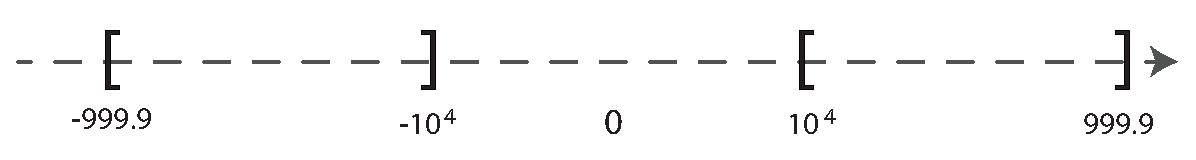
\includegraphics[scale=.7]{dominio-linha.eps}

\vspace{\fill}

*IEEE 754 : F(2,23,-127,128)

\newpage

\subsection{Erros}

\subsubsection{Erros absolutos e relativos}

\begin{align*}
	&x: \textrm{Valor exato}\\
	&\overline{x}: \textrm{Valor aproximado de x}\\
	&Def : \textrm{Erro absoluto }EA_x = x-\overline{x}\\
	&\lvert EA_x \rvert \ge 0\\
	&Def :\textrm{Erro relativo }ER_x = \frac{EA_x}{\overline{x}}
\end{align*}

Exemplo:
\begin{align*}
	&x\in (2112.8,2113) \; \overline{x}=2112.9\\
	&y \in (5.2,5.3) \; \overline{y}=5.3\\
	\\
	&\lvert EA_x \rvert < 0.1\\
	&\lvert ER_x \rvert < 4.7\times 10^{-5}\\
	&\lvert EA_y \rvert < 0.1\\
	&\lvert ER_y \rvert < 0.02	
\end{align*}
Representação de x por $\overline{x}$ é relativamente mais precisa do que y por $\overline{y}$

\subsubsection{Erro de arredondamento e truncamento}
\begin{align*}
B &= 10 , t \textrm{ digitos}\\
x &= 0. d_1 d_2 ... d_t \times 10^e\\
&= 0. d_1 d_2 ... d_{t-1} \times 10^e\\
& + 0. 000...0 d_t \times 10^e\\
&= 0. d_1 d_2 ... d_{t-1} \times 10^e + 0. d_t \times 10^{e-t}\\
&:= f_x \times 10^e + g_x \times 10^{e-t}
\end{align*}

Exemplo:
\begin{align*}
	t=4,x&=234.57\\
	&= 0.2345\times 10^3 +0.7 \times 10^{-1}\\
	&= f_x \times 10^3 + g_x \times 10^{-1}
\end{align*}

\begin{enumerate}
	\item Truncamento\\
	\begin{align*}
		&g_x \leftarrow 0 , \overline{x} \leftarrow f_x\times 10^e\\
		&\lvert EA_x \rvert < 10^{e-t}\\
		&\lvert ER_x \rvert < 10^{-t+1}
	\end{align*}
	\item Arredondamento\\
	\begin{enumerate}[a)]
		\item $\lvert g_x \rvert < \frac{1}{2}$
		\begin{align*}
			g_x \leftarrow 0, \overline{x} &= f_x \times 10^e,\\
			&\lvert EA_x \rvert < \frac{1}{2} \times 10^{e-t}\\
			&\lvert ER_x \rvert < \frac{1}{2}\times 10^{-t+1}		
		\end{align*}
		\item $\lvert g_x \rvert \ge \frac{1}{2}$
		\begin{align*}
			g_x &\leftarrow 10^{e-t},\\
			\overline{x} &= f_x \times 10^e + 10^{e-t},\\
			&\lvert EA_x \rvert \le \frac{1}{2} \times 10^{e-t}\\
			&\lvert ER_x \rvert < \frac{1}{2} \times 10^{-t+1}		
		\end{align*}		 
	\end{enumerate}
	$\longrightarrow \lvert EA_x \rvert \le \frac{1}{2}\times 10^{e-t},\; \lvert ER_x \rvert < \frac{1}{2}\times 10^{-t+1}$
\end{enumerate}

\subsubsection{Propagação de erros em sequências de operações aritméticas}

\begin{enumerate}
	\item Propagação dos erros dos operandos
	\begin{enumerate}[a)]
		\item Adição
		\begin{align*}
			&\textrm{Ex: }F(10,4,-3,3)\\
			X&=1.3749213 \textrm{ Valor exato}\\
			\overline{X} &= 0.1374 \times 10^1 \;\;\;\;\; EA_x = X - \overline{X} = 0.0009213...\\
			Y &= 573.27482\\
			\overline{Y} &= 0.5732\times 10^3 \;\;\;\;\; EA_y = Y = \overline{Y} = 0.0007482\\			
		\end{align*}
		\begin{align*}
			&X+Y = \overline{X} + \overline{Y} + EA_X + EA_Y\\
			&\bigoplus \textrm{: Operação de adição no sistema de ponto flutuante}\\
			&\overline{X} \bigoplus \overline{Y}\textrm{($EA_x + EA_y$ desconhecidos)}\\
			&= \overline{\overline{X}+\overline{Y}}\\
			&\frac{0.0013\times 10^3}{0.5732\times 10^3}=0.5745\times 10^3 \textrm{(somente quatro casas na mantissa)}\\
			&\overline{X}+\overline{Y} = 1.374 + 573.2 = 574.574\\
			&\overline{\overline{X}+\overline{Y}} = 574.5\\
			&EA_{\overline{x}+\overline{Y}}=\overline{X}+\overline{Y} - \overline{\overline{X}+\overline{Y}} =0.074\\						
		\end{align*}
		$X+Y= 574.6497413$ Vs %$\overline{\overline{X}+\overline{Y}} = 574.5$\\
		\item Operações:
		\begin{center}
		\begin{tabular}{| c | c | c |}
				\hline
				Operação & Erro abs. & Erro rel. \\
				\hline
				Adição & $EA_{x+y} = EA_x + EA_y$ & $ER_{x+y} = ER_x  \times \frac{\overline{x}}{\overline{x}+\overline{y}} + ER_y  \times \frac{\overline{y}}{\overline{x}+\overline{y}}$ \\
				Subtração & $EA_{x-y} = EA_x - EA_y$ & $ER_{x-y} = ER_x  \times \frac{\overline{x}}{\overline{x}-\overline{y}} - ER_y  \times \frac{\overline{y}}{\overline{x}-\overline{y}}$ \\
				Multiplicação & $EA_{xy} \approx  \overline{x}\times EA_y + \overline{y}\times EA_x$ & $ER_{xy} \approx ER_x + ER_y$\\
				Divisão & $EA_{\frac{x}{y}} \approx \frac{\overline{y} EA_x - \overline{x}EA_y}{\overline{y}^2}$ & $ER_{\frac{x}{y}} \approx ER_x - ER_y$\\
				\hline
			\end{tabular}
		\end{center}
	\end{enumerate}
\end{enumerate}

\chapter{Resolução de Sistemas Lineares}
Sistema Linear: m equações lineares em n variáveis\\
  Variavel:$x_j$	$j =1,...,n$\\
  Equação: $i \rightarrow a_{i1}x_1 + a_{i2}x_2 + ... + a_{in}x_n = b_1$\\
  
  Em cálculo numérico levaremos em conta na maioria o caso m = n
  
  Em forma matricial temos: $Ax=b$\\
  com
  \begin{align*}
  	A=
  	\begin{bmatrix}
  	a_{11}  & a{12}  & \cdots & a_{1n} \\
  	\vdots  & \vdots  & \vdots & \vdots \\
  	a_{n1} & a_{n2} & \cdots & a_{nn} 
  	\end{bmatrix}
  	\;
  	x = 
  	\begin{bmatrix}
  	x_1\\ \vdots \\ x_n
  	\end{bmatrix}
  	\;
  	b = 
  	\begin{bmatrix}
  	b_1 \\ \vdots \\ b_n
  	\end{bmatrix}
  \end{align*}
  
  Problema em questào: Dado A e b determinar x.\\
  
  \section{Métodos Diretos}
  \subsection*{Regra de Cramer}
  \begin{align*}
  x_i = \frac{det(A_i)}{det (A)}
  \end{align*}
  det: Determinante\\
  $A_i$: Substituição da coluna i por b em A\\
  Esse método se torna extremamente complexo para n >> 2, pois se houver n+1 determinantes de ordem n, teremos: $(n+1)\times n!\times (n-1)$ multiplicações\\
  Com n = 20  um computador que faça 100 milhões de multiplicações por segundo levaria 300.000 anos para computar.
  \subsection*{Inversa}
  $Ax=b \longrightarrow A^{-1}Ax=A^{-1}b \longrightarrow x = A^{-1}b$ caso $A^{-1}$ exista.\\
  Problemas: ineficiente e instável (graças ao erro de arredondamento existente nas inversões, que se acumulam).
  \subsection*{Resolução de SL Triangulares}
  Dado a matrix A triangular superior n x n com elementos diagonais $a_{ii}$ não nulos.
  
  A = 
  $\begin{bmatrix}
  a_11 & a_12 & \cdots & a_{1n}\\
  0 & a_22 & \cdots & a_{2n}\\
  0 & 0 & \ddots & \ddots \\
  0 & 0 &\cdots & a_{nn}
  \end{bmatrix}$
  
  \begin{algorithmic}
  \STATE $x_n = b_n/a_{nn}$
  \FOR {$k=n-1,...,1$}
  \STATE soma = $b_k$
  \FOR {$j=k+1,...,n$}
  \STATE soma = soma - $a_{kj}x_j$
  \ENDFOR
  \STATE $x_k = \frac{soma}{a_{kk}}$
  \ENDFOR
  \end{algorithmic}
  
  
  Esforço computacional:\\
  n 	divisões\\
  $\sum_{j=1}^{n_1} j = n(n-1)/2$	adições\\
  $\sum_{j=1}^{n-1} j =n(n-1)/2$	multiplicações\\
  Gerando uma complexidade $O(n^2)$ (a mesma do bubblesort)
 \end{document}
